%======================================================================
\chapter{Zupply Framework Implementation}\label{ch:zupply_implementation}
%======================================================================

\section*{Declaration of Contributions}
This chapter is based on~\cite{Badakhshan2024Zupply} and~\cite{Badakhshan2025AuroraZupply}. I am the sole author of this chapter under the supervision of Professor Guang Gong.

\section{Introduction}

In the previous two chapters, we introduced the design and security analysis of the Zupply framework. This chapter focuses on its implementation, detailing the 
% construction of \gls{r1cs} instances, the 
instantiation of core building blocks, and the implementation of the zero-knowledge proving and verification algorithms. Specifically, we describe the arithmetic circuits for the \gls{np} problems associated with \textsf{Auth}, \textsf{Trans}, \textsf{Merge}, and \textsf{Div}. These circuits generate \gls{r1cs} instances in a manner that enables succinct zero-knowledge proofs (\gls{zkp}s) while preserving confidentiality. To optimize on-chain costs (i.e., smart contract execution) we minimize the public inputs to these circuits. 
We provide two implementation variants of Zupply based on its \gls{zkp} algorithms. The first employs Groth16 \cite{Groth2016} \gls{zksnark} over BN254 \cite{BNcurve} and BLS12-381~\cite{BLS_curve2003} elliptic curves, accommodating different security levels. The second leverages Aurora~\cite{Aurora2019}, a \gls{zksnark} designed for a transparent setup and post-quantum security against quantum-capable malicious provers.

Zupply is implemented in \CC and Solidity, demonstrating both computational and cost efficiency. This development validates the framework's practicality for real-world applications. While directed acyclic graphs (\gls{dag}s) are widely used for maintaining product histories in supply chains, Zupply's utility extends beyond this domain. We show that Zupply provides a practical, cost-efficient, and privacy-preserving solution for decentralized supply chain management (\gls{scm}) systems.

\section{Zupply Arithmetic Circuits}
\label{sec:Zupply Arithmetic Circuits}

\begin{figure*}
    \centering
    \begin{subfigure}[b]{0.35\textwidth}  % Adjusted to fit four images in one row
        \centering
        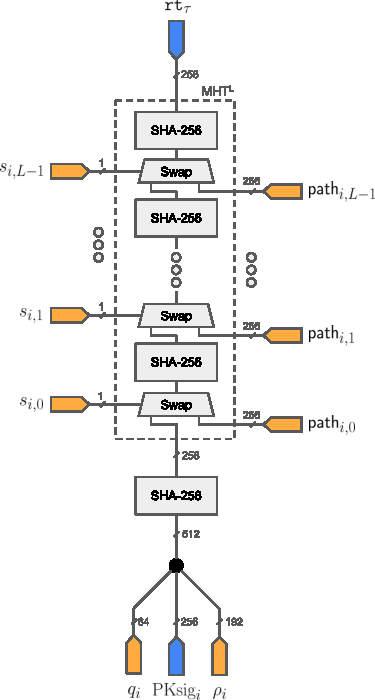
\includegraphics[scale=0.6]{Figures/Auth.pdf} % Replace with your image file
        \caption{\textsf{Auth} circuit}
        \label{fig:Authcircuits}
        
    \end{subfigure}
    \hfill
    \begin{subfigure}[t]{0.60\textwidth}  % Adjusted to fit four images in one row
        \centering
        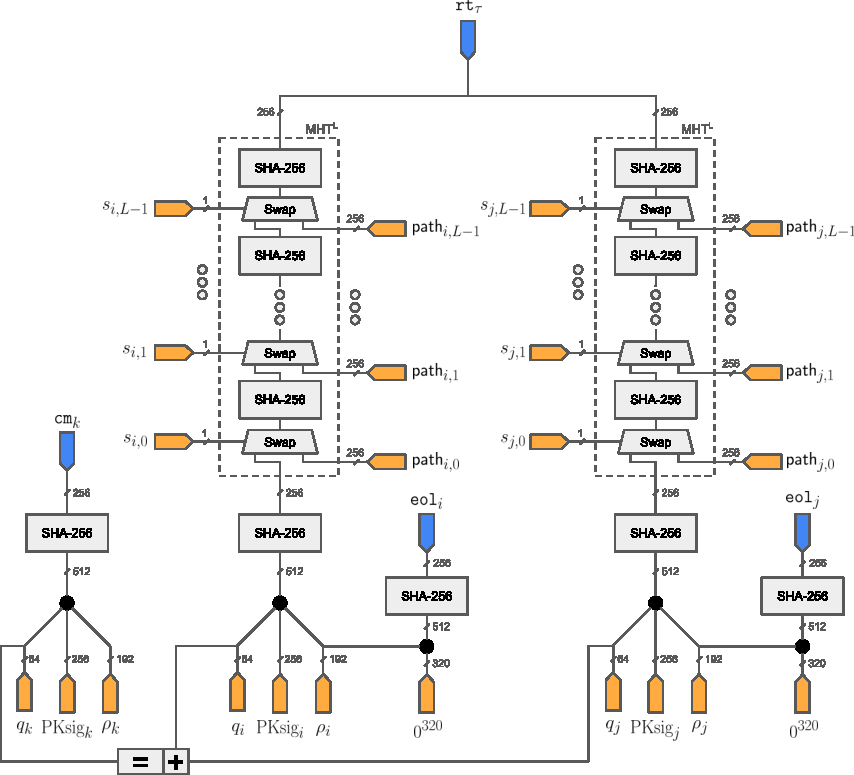
\includegraphics[scale=0.6]{Figures/Merge.pdf} % Replace with your image file
        \caption{\textsf{Merge} circuit}
        \label{fig:Mergecircuits}
    \end{subfigure}
    \hfill\vspace{5mm}
    \begin{subfigure}[t]{0.35\textwidth}  % Adjusted to fit four images in one row
        \centering
        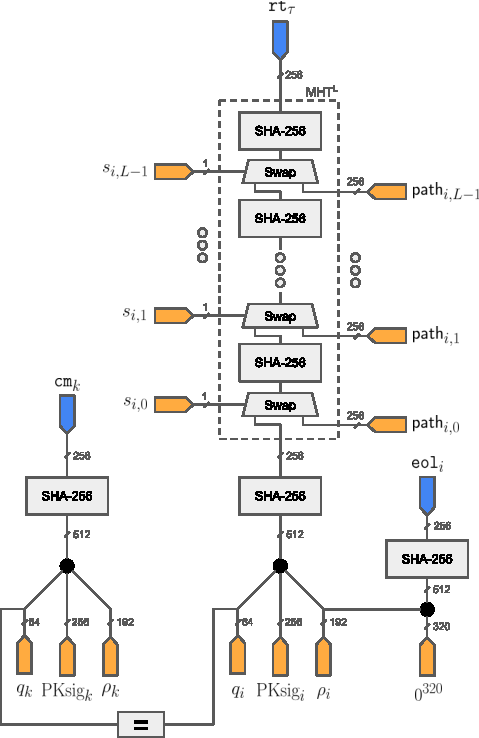
\includegraphics[scale=0.6]{Figures/Trans.pdf} % Replace with your image file
        \caption{\textsf{Trans} circuit}
        \label{fig:Transcircuits}
        
    \end{subfigure}
    \hfill
    \begin{subfigure}[t]{0.60\textwidth}  % Adjusted to fit four images in one row
        \centering
        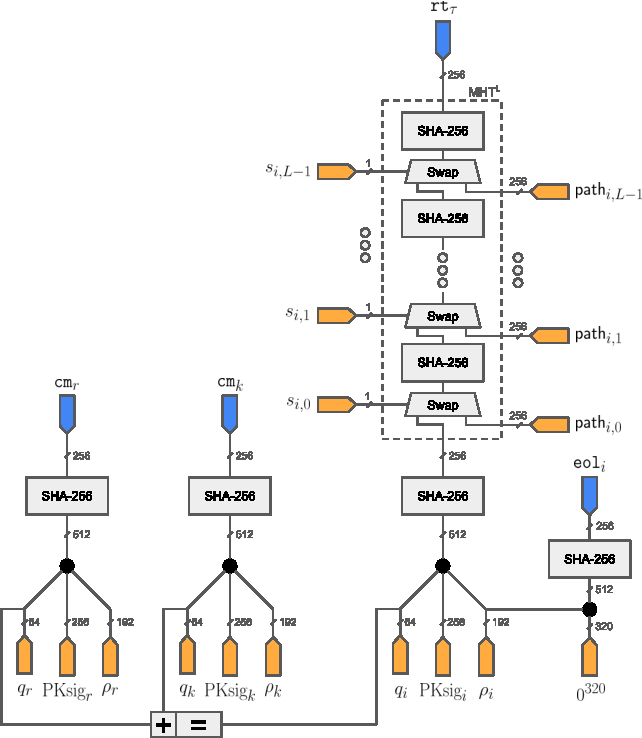
\includegraphics[scale=0.6]{Figures/Div.pdf} % Replace with your image file
        \caption{\textsf{Div} circuit}
        \label{fig:Divcircuits}
        
    \end{subfigure}
    
   \caption[Zupply arithmetic circuits]{Schematic representation of the arithmetic circuits for \gls{zkp}s in the Zupply framework. The Merkle hash tree has a depth of $L$, with public inputs highlighted in \textcolor{blue}{\textbf{blue}}. Inputs highlighted in \textcolor{orange}{\textbf{orange}}, along with the intermediate values within the arithmetic circuits, are private (auxiliary) inputs. The hash function used in the implementation is SHA-256.}
    \label{fig:circuits}
\end{figure*}


The \textsf{Auth}, \textsf{Trans}, \textsf{Merge}, and \textsf{Divide} algorithms in the Zupply framework generate \gls{zkp}s to demonstrate knowledge of the pre-image for one or two commitments to anonymous authentication tokens (\gls{aat}s) in the Merkle hash tree (\textsf{MHT}), with the root at time $\tau$ is denoted by $\texttt{rt}_\tau$. These \gls{zkp}s are used in Zupply algorithms to prove ownership of an \gls{aat} for authenticating a data record or to transfer ownership of the \gls{aat}s. In all cases, the prover avoids revealing the \gls{aat} or its commitment stored in the \textsf{MHT}. Figure \ref{fig:circuits} shows a schematic view of the arithmetic circuits associated with each of these \gls{zkp}s.


These circuits represent the \gls{np} problem related to each \gls{zkp} and are converted into \gls{r1cs}, which are satisfied only when the prover provides consistent inputs to the constraint system. For example, in a circuit designed to prove knowledge of the pre-image of a leaf in a Merkle hash tree with root \texttt{rt}, without revealing the specific leaf, the root of the Merkle hash tree is given as a public input. The private inputs include the corresponding leaf pre-image and the Merkle proof. These private inputs must align with the root and satisfy the circuit constraints. As a result, the prover must provide valid private inputs, thereby demonstrating knowledge of the pre-image of a leaf in the Merkle hash tree.
In the Zupply framework, the root value is determined by the shared \textsf{MHT}, which is maintained within the framework and serves as a public input to the circuits. The prover must demonstrate knowledge of the pre-image of a leaf in the fully decentralized \textsf{MHT}. Importantly, this process does not reveal any information about the \gls{aat} or its commitment (the leaf itself).



Each arithmetic circuit in the Zupply framework includes a proof of knowledge for one or two leaves within the \textsf{MHT}. These circuits are constructed using the arithmetic circuits for the hash function and the Merkle hash tree. The \gls{r1cs}  generated by the hash function arithmetic circuit is satisfied if and only if, for a given input value $x$ assigned to the circuit, the output value $y$ satisfies $y = \mathcal{H}(x)$, where $\mathcal{H}$ is the hash function.
The arithmetic circuit of the Merkle hash tree implements the Merkle proving algorithm. At each level, a hash function output is concatenated to either the left or right of its adjacent hash. The concatenated value is then input to the hash function of the subsequent layer, continuing until the root is reached. Formally, this chain of hash functions is expressed as:
\[
h_{i,j+1} = \mathcal{H}\left( s_{i,j}\cdot(h_{i,j} \,|\ \textsf{path}_{i,j}) + (1-s_{i,j})\cdot(\textsf{path}_{i,j} \,|\ h_{i,j}) \right),
\]
where at layer $j$, $h_{i,j}$ is the output from the previous hash in the chain. Let $h_{i,0}$ denote the $i$-th leaf value and $h_{i,L}$ is equal to the root \texttt{rt}. $\textsf{path}_{i,j}$ represents the adjacent hash at layer $j$ in the Merkle proof related to index $i$, and $s_{i,j} \in \{0,1\}$ determines whether $h_{i,j}$ is concatenated to the left or right of its adjacent hash. 
The arithmetic circuit responsible for managing this order selection is called the ``Swap'' block. The \gls{r1cs}  generated by the arithmetic circuit of a Merkle hash tree with $L$ layers is satisfied if and only if the leaf $h_0$ exists in a Merkle hash tree with root \texttt{rt}, and the Merkle proof, comprising $\{\textsf{path}_{i,0}, \dots, \textsf{path}_{i,L-1}\}$ and $\{s_{i,0}, \dots, s_{i,L-1}\}$, is consistent with both the leaf and the root.


In the following, we delve into the details of each circuit.



\subsection{\textsf{Auth} Circuit} 
The \textsf{Auth} circuit, illustrated in Figure \ref{fig:Authcircuits}, generates the \gls{zkp} $\pi_\textsf{Auth}$, which is embedded in data records to prove that the data creator possesses an \gls{aat} within a Merkle hash tree. The root $\texttt{rt}_\tau$ serves as a public input to this proof to allow the auditor to verify that the commitment to the claimed \gls{aat} is stored in the \textsf{MHT} with root $\texttt{rt}_\tau$. Specifically, the prover asserts, ``she knows a preimage of one of the commitments to an \gls{aat} in the \textsf{MHT} with root $\texttt{rt}_\tau$,'' without revealing which commitment. Additionally, the PKsig associated with the \gls{aat} is also provided as a public input. The data creator signs the data record using the corresponding SKsig, thereby proving that the data has been signed by the token owner and remains unaltered.


\subsection{\textsf{Trans} Circuit} 
The \textsf{Trans} circuit generates the \gls{zkp} $\pi_\textsf{Trans}$, which is submitted to the blockchain platform when an entity transfers ownership of an \gls{aat} during \textsf{OT-Protocol}. Specifically, it obsoletes an \gls{aat} owned by the entity and creates a new \gls{aat} that is consistent with the obsoleted \gls{aat}. The circuit used for generating this proof is depicted in Figure \ref{fig:Transcircuits}.  In the \textsf{Trans} circuit, the pre-images of the commitments to both the new and obsoleted \gls{aat}s are private inputs. The circuit ensures that the $q$ value, representing the quantity of the product, remains unchanged. The commitment to the new \gls{aat} serves as a public input to the circuit, which will be added to the \textsf{MHT}. Additionally, the end of life (\texttt{eol}) value of the obsoleted \gls{aat} is a public input to the circuit and is published on the blockchain platform. This ensures that an entity cannot reuse an \gls{aat} included in the \textsf{MHT} but transferred before. In this proof, the prover asserts: ``She knows an \gls{aat} in the \textsf{MHT} with root $\texttt{rt}_\tau$, where the end-of-life value of the claimed token is \texttt{eol}, and she has created a new \gls{aat} with a commitment \texttt{cm}, such that the quantity in the new token matches the quantity in the originally claimed token.''



\subsection{\textsf{Merge} Circuit} 
The \textsf{Merge} circuit is similar to the \textsf{Trans} circuit, but it merges two existing commitments to two known \gls{aat}s in \textsf{MHT} with root $\texttt{rt}$. Hence, this circuit generates the \gls{zkp} $\pi_\textsf{Merge}$ which proves the knowledge of two \gls{aat}s, where their corresponding \texttt{eol}s are public inputs to this circuit, allowing the verification algorithm to check whether those \gls{aat}s have been transferred before. This circuit also guarantees that the quantity of the product in the new commitment is equivalent to the sum of the product quantities in the two preceding \gls{aat}s. The new commitment to the new \gls{aat} is a public input to this circuit.


\subsection{\textsf{Div} Circuit} 
The \textsf{Div} circuit is the opposite of the \textsf{Merge} circuit. It generates the \gls{zkp} $\pi_\textsf{Div}$, which proves that a known existing \gls{aat} in \textsf{MHT} with root $\texttt{rt}$ divides into two new \gls{aat}s. The \texttt{eol} of the divided token and the commitments to the two new \gls{aat}s are public inputs to this circuit. This circuit ensures consistency in the product quantity before and after division, so that the sum of the $q$ values in the new tokens equals the $q$ value in the original \gls{aat}.


\section{Cryptographic Primitives and Parameters} \label{sec:zupply_primitive_and_parameters}
In this section, we present the instantiation of each building block  of the Zupply framework, considering a 128-bit security level. 

\subsection{Blockchain platform }
Ethereum provides the highest level of security among all ethereum virtual machine (\gls{evm}) compatible blockchains, such as Arbitrum and Avalanche \cite{Neiheiser2023PracticalLimitations, Kalodner2018Arbitrum, Avalanche}. Therefore, we have selected Ethereum as the blockchain platform upon which Zupply is built. If Zupply remains practical with respect to the costs incurred when calling the smart contract $\mathcal{C}_Z$, then its feasibility extends to other \gls{evm}-compatible blockchains as well. To realize the proof-of-inclusion ($\mathbf{L}_\tau^\mathsf{PI}(\texttt{rt})$), Ethereum employes Merkle Patricia tree (trie) \cite{PatriciaTree, ethereum} and provides $\texttt{eth\_getProof}$ API which is elaborated in EIP-1186 \cite{Jentzsch2018}. 


\subsection{Decentralized Cloud Storage (DCS)}

Zupply utilizes the 
InterPlanetary File System
(\gls{ipfs}) network \cite{Benet2014} for file storage, offering flexibility in data management based on the preferences of the supply chain entities. For instance, entities can opt to share their data records directly from their computers via a Tor hidden service \cite{Loshin2013PracticalAnonymity} to obscure their IP address, or they can entrust storage to major stakeholders within the suppl 	y chain. These stakeholders then anonymously publish the data records to the \gls{ipfs} network, ensuring availability. Furthermore, Zupply guarantees the authenticity and integrity of data records, which are independently verified by auditors, thus eliminating reliance on \gls{dcs} for this verification. 
% Moreover, integrity is maintained as any data alteration causes the \textsf{Audit} algorithm to return a 0, effectively detecting tampering. 


%as detailed in Definition \ref{def:informal-Authenticity}, 


% Filecoin \cite{filecoin}, a decentralized storage network based on IPFS \cite{ipfs}, is considered a potential candidate for DCS. 
 
% Therefore, we can employ different kinds of instantiations. 



\subsection{Collision-resistance Hash Function}

The collision resistance hash function $\mathcal{H}$ is a 512-bit input to a 256-bit output mapping; namely, $\mathcal{H}:\{0,1\}^{512} \rightarrow \{0,1\}^{256}$. It can be implemented by either SHA-256 or SHA3-256. For SHA-256, it has 512 bit input and 256 output, so there is no padding bits needed. For SHA3-256, the input size is 1088 bits  and outputs 256 bits. So, in this case, padding is needed. In our implementation, we selected SHA-256 for its simplicity and wide adoption.  

\subsection{Statistically-hiding Commitment}
We instantiate the commitment scheme \textsf{COMM} via $\mathcal{H}$. Such that 
% for computing the commitment to $\Tilde{T} := (q, \text{PKsig}, \rho)$, 
$\texttt{cm}:=\mathsf{COMM}_\rho(\Tilde{T}) = \mathcal{H}(q||\text{PKsig}||[\rho]_{224})$
Where, $q \in \{0, 1\}^{32}$, $\text{PKsig} \in \{0, 1\}^{256}$, and $\rho \in \{0, 1\}^{512}$. Moreover, $[\rho]_{224}$ denotes that the $512$-bit $\rho$ is truncated to $224$ bits by dropping most significant bits. Both $\text{PKsig}$ and $\rho$ 
% (which is the output of a cryptographically strong random number generator (RNG) \cite{NISTPRNG}) 
can serve as randomness for the commitment. 
% Operator $\xleftarrow{R}$ is a cryptographically strong random number generator (RNG) \cite{NISTPRNG}.  The Digital signature algorithm used in the experiment is  the curve Secp256k1 \cite{brown2009standards}.

\subsection{Merkle Hash Tree}
\textsf{MHT} is constructed based on the collision resistance hash function $\mathcal{H}$ (i.e., SHA-256). Let the number of layers $L$ be equal to 20, then \textsf{MHT} has $2^{20} -1$ nodes, and each node has 256 bits. Consequently, the tree requires 32 MB of storage. Recall that the tree is stored off-chain on entities' $\textsc{Z-Node}$ software, and only the root \texttt{rt} is maintained on the smart contract $\mathcal{C}_Z$.


\subsection{Strongly-unforgeable Digital Signature}

The signature scheme algorithm \textsf{Sig} used in the framework is Elliptic Curve Schnorr signatures (EC-Schnorr) \cite{Schnorr1991Signature} over the elliptic curve secp256k1 \cite{sec2_2010} where the size of both PKsig and SKsig are 256 bits and signature has 512 bits. The algorithm uses SHA-256 as the hash function required for the signatures. This algorithm satisfies the \textit{SUF-CMA} security property.

% \subsection{Public-key encryptions}
% Zupply framework employs Elliptic Curve Integrated Encryption Scheme (ECIES) over secp256k1 \cite{sec2_2010} for $\mathsf{Enc}$. This algorithm enables 256-bit PKenc and SKenc keys and satisfies \textit{IND-CCA} security property \cite{katz2020introduction}.

\subsection{Symmetric-key Encryption}
For \textsf{SymEnc}, we use 128-bit advanced encryption standard (AES-128) algorithm in cipher block chaining (CBC) mode which satisfies \textit{IND-CPA} security property \cite{rogaway2011evaluation, sibleyras2020Security}.

\section{zkSNARK Instantiations}
The choice of \gls{zksnark} protocol in the Zupply framework enables a trade-off between computational efficiency and enhanced security properties, such as post-quantum security and a transparent setup.

\subsection{Groth16}

In the first implementation variant of the Zupply framework, we employ Groth16 \cite{Groth2016}, a \gls{zksnark} known for generating succinct proofs and enabling fast verification. This protocol is a pairing-based \gls{zksnark} for \gls{r1cs}. The scheme requires a trusted setup phase that can be done via a secure multi-party computation (\gls{smpc}) \cite{Ben-Sasson2015SecureSampling, Nikolaenko2024PowersofTau}.
We evaluate the implementation using two elliptic curves: BN254 \cite{BNcurve}, offering the fastest algorithms and the smallest proof sizes and approximately 100-bit security \cite{Barbulescu2019}, and BLS12-381 \cite{BLS_curve2003}, designed for 128-bit security.


By using the Groth16 \gls{zksnark} in the Zupply framework, the verification keys ($\text{vk}_\mathbbm{x}$), stored in $\mathcal{C}_Z$, remain small when the number of public inputs ($x_\mathbbm{x}$) is minimal. Additionally, the verification algorithm ($\mathsf{Verify}$) of Groth16 is less complex compared to other \gls{zksnark}s. Due to the high cost of on-chain storage, this efficiency makes Groth16 particularly suitable for public blockchains where execution and storage costs are high.
In Groth16, the proof size remains constant regardless of the number of constraints in the associated \gls{r1cs}. The proof is denoted as \(\pi \in \mathbb{G}_1^2 \times \mathbb{G}_2\), where \(\mathbb{G}_1\) consists of points on the elliptic curve, and \(\mathbb{G}_2\) comprises points on a twist of the curve.  

The size of the verification key \(\textsf{vk}\) depends on the number of public inputs in each \gls{r1cs} instance within the Zupply framework. The public input of the instances in the Zupply framework are denoted as \(x_\mathsf{Auth}\), \(x_\mathsf{Trans}\), \(x_\mathsf{Merge}\), and \(x_\mathsf{Div}\).
Let \(|x_\mathbbm{x}|\) represent the number of public inputs for an instance \(\mathbbm{x}\). As described in \cite{Groth2016}, \(\textsf{vk}\) consists of \(|x_\mathbbm{x}| + 2\) elements in \(\mathbb{G}_1\) and three elements in \(\mathbb{G}_2\). It may also include a precomputed element in \(\mathbb{G}_T\) via the bilinear pairing \( e: \mathbb{G}_1 \times \mathbb{G}_2 \to \mathbb{G}_T \) applied to two specific elements in \(\textsf{vk}\), since the verification process requires only their pairing, not those elements themselves. Consequently, one element from each of \(\mathbb{G}_1\) and \(\mathbb{G}_2\) can be omitted from \(\textsf{vk}\) and replaced by an element in \(\mathbb{G}_T\).

In the Zupply framework, every public input is represented as either a 256-bit hash or a 256-bit public key. However, like other scalar elements in \gls{r1cs} instances, these inputs must belong to the scalar prime field of the underlying elliptic curve. Since the scalar numbers in BN254 and BLS12-381 have bit-lengths of 254 and 255 bits, respectively, each 256-bit value is split into two 128-bit public inputs to minimize the public input size. In contrast, the original implementation of the SHA-256 arithmetic circuit in \cite{libsnark} treats each 256-bit hash as 256 distinct public inputs, significantly increasing the size of the verification keys. Based on our construction, the number of public inputs represented as $n(x_\mathbbm{x})$ in Table \ref{tab:zksize} are double the count of public inputs as per the arithmetic circuits presented in Section \ref{sec:Zupply Arithmetic Circuits}. Moreover, the size of the proving key \textsf{pk} is determined by the number of constraints in each instance and the proving keys in the Zupply framework are stored off-chain on the devices of entities. The number of constraints is determined by the size of the circuit implementing \gls{np} statements in Section \ref{sec:Zero-knowledge Proofs}. 

\subsubsection{Over BN254 Curve}
We initially implement the Groth16 \gls{zksnark} over the BN254 curve. The curve was generally assumed to offer around 128 bits of security \cite{BNcurve}; However, research by Kim et al. \cite{Kim2015Extended} suggests that its actual security level might be lower. In Groth16, the proof size is constant, denoted as \(\pi \in \mathbb{G}_1^2 \times \mathbb{G}_2\), where \(\mathbb{G}_1\) consists of points on the BN254 elliptic curve, and \(\mathbb{G}_2\) comprises points on a twist of the BN254. Consequently, the proof size is 128 bytes, regardless of the size of the number of constraints in the \gls{r1cs} related to the proof.
Since Ethereum only provides pre-compiled contracts for the BN254 curve \cite{EIP197, Housni2022Families}, we selected this pairing-friendly curve for the on-chain Groth16 verification algorithms implementation. 

\subsubsection{Over BLS12-381 Curve}
To strengthen the security of our framework, we replace the BN254 curve with BLS12-381, which offers 128-bit security. However, as of the time of writing, Ethereum does not provide precompiled support for operations over this curve \cite{Vlasov2020}. Consequently, we did not implement our smart contract $C_\mathcal{Z}$ using BLS12-381, leaving this for future work. Adopting this curve increases the proof size to 192 bytes regardless of the size of the number of constraints in  \gls{r1cs}. Table \ref{tab:zksize} compares the verification and proving key sizes for each instance in Zupply using both the BN254 and BLS12-381 curves.

\begin{table}
 \caption[Comparison of the Groth16 key sizes for each NP statement in Zupply]{Comparison of verification and proving key sizes of Groth16 \gls{zksnark} for \gls{np} statements in the Zupply framework for $L=20$. $\nu = n(x_\mathbbm{x})$ is the number of public inputs, $N$ is the number of constraints, $|\mathsf{vk}_\mathbbm{x}|$ is the size of the verification key in Bytes, and  $|\mathsf{pk}_\mathbbm{x}|$ is the size of the proving key in MegaBytes.}
	\centering

\begin{tabular}{ccccccc}
		\toprule
		\multirow{2}{*}{\textbf{$\mathbbm{x}$}} & \multirow{2}{*}{\textbf{$\nu$}} & \multirow{2}{*}{$N$} & \multicolumn{2}{c}{$|\mathsf{vk}_\mathbbm{x}|$ (B)} & \multicolumn{2}{c}{$|\mathsf{pk}_\mathbbm{x}|$ (MB)} \\
		% \cline{4-7}
		 &  &  & {\footnotesize BN254} & {\footnotesize BLS12-381} & {\footnotesize BN254} & {\footnotesize BLS12-381} \\
		\midrule
        Complexity & - & $O(L)$ & \multicolumn{2}{c}{$O(\nu)$}  & \multicolumn{2}{c}{$O(N)$}\\
        
		${\textsf{Auth}}$ & 4  & 588,248  & 768 & 1,152 & 182.5 & 456.3\\
		
		${\textsf{Trans}}$ & 6  & 642,876  & 896 & 1,344 & 200 & 246.75\\
		${\textsf{Merge}}$ & 8 & 1,258,337  & 1,024 & 1,536 & 393.8 & 447.93\\
		${\textsf{Div}}$ & 8 & 670,091  & 1,024 & 1,536 & 210 & 262.5\\
		\bottomrule
	\end{tabular}
	\label{tab:zksize}
\end{table}

\subsection{Aurora}

In the first implementation variant of the Zupply framework, we employ Aurora \cite{Aurora2019}. It is a \gls{zksnark} protocol  that offers transparent-setup, which eliminates the necessity for a trusted parties in the setup phase. Aurora is built upon particularly the Interactive Oracle Proofs (\gls{iop}s) \cite{Ben-Sasson2016IOP} for \gls{r1cs} obtained by the Fast Reed-Solomon Interactive Oracle Proof of Proximity (\gls{fri}) protocol for low degree testing \cite{FRI2018}. Aurora notably avoids dependence on hard mathematical problems such as discrete logarithms or integer factorization, which makes Aurora plausibly post-quantum secure. Aurora relies on minimal assumptions as it requires only a collision-resistant hash function. This makes it a suitable choice for transitioning the Zupply framework toward enhanced post-quantum security.


Since the \gls{r1cs} constraints generated for the Zupply framework in the previous implementation have their elements in the scalar field associated with the chosen elliptic curve, we used the Aurora implementation over the same finite fields and on multiplicative groups. But, Aurora can also be used over binary extension fields and additive groups, which can make its computations faster due to simpler arithmetic operations and reduced computational overhead. We chose the former configuration for compatibility with the first implementation.




\section{Software Implementation}

In this section, we provide a detailed overview of the \CC software implementation\footnote{The implementation is available at \url{https://github.com/mtbadakhshan/zupply-zkp}} for each variant discussed above. Additionally, we introduce a baseline model for comparison, which does not incorporate privacy preservation. 

\subsection{Baseline Model}
To assess the cost overhead introduced by privacy preservation using \gls{zkp}s in the Zupply framework for a supply chain management (\gls{scm}) application, we propose a non-privacy-preserving baseline model that maintains the same functionality; specifically, (non-anonymous) authentication tokens for off-chain data uploading. In the baseline model's smart contract, a token owned by an entity $e_i$ holds $e_i$'s address ($\text{BPAddr}^{e_i}$) and is only transferable by $e_i$. Furthermore, each token holds a quantity, enabling the merging and dividing of tokens. The token owner $e_i$ can use the private key corresponding to $\text{BPAddr}^{e_i}$ to sign off-chain data records, as explained in ERC-4361 \cite{ERC-4361}, or transfer the token.

\subsection{Groth16 Based Implementation}
For the Groth16 \gls{zksnark} instantiation, we employed libsnark \cite{libsnark}, a \CC library developed by SCIPR lab \cite{SCIPR}, which offers implementations of the Groth16 \gls{zksnark} scheme for provers and verifiers. This library was instrumental in generating \gls{r1cs} constraints for \gls{np} problems within our framework, achieved by implementing them as arithmetic circuits. Additionally, to integrate the Groth16 verification algorithm into $\mathcal{C}_Z$, we utilized the ZoKrates \cite{ZoKrates} toolbox. As previously discussed, we only provide the Zupply smart contract implementation using Groth16 over BN254. 

Table \ref{tab:transaction_gas} presents the costs associated with executing transactions in both the Zupply framework and the baseline model on the Ethereum blockchain. 
At the time of deploying $\mathcal{C}_Z$, some one-time costs should be paid as it uploads the code, a 256-bit \texttt{rt}, and all verification keys except $\mathsf{vk}_\mathsf{Auth}$ to blockchain. $\mathsf{vk}$ sizes are listed in Table \ref{tab:zksize}.  Transactions $\texttt{tx}_\mathsf{Trans}$, $\texttt{tx}_\mathsf{Merge}$, and $\texttt{tx}_\mathsf{Div}$ execute \textsf{VerifyTX} on  $\mathcal{C}_Z$ and contain a 256 bytes $\pi$, one or two $20 \times 256$ bits $\mathsf{path}$ (for $L=20$), new $256$-bit \texttt{rt}s,  $256$-bit \texttt{cm}s, and $256$-bit \texttt{eol}s. 
While the deployment cost is a one-time expense, entities incur transaction fees each time they transfer products to the next entity. 

We also implemented the zero-knowledge proving and verification algorithms of the Zupply framework using Groth16 over the BLS12-381 curve. Consequently, the elements in the \gls{r1cs} constraint system are in the scalar prime field associated with the BLS12-381 curve.

\subsection{Aurora Based Implementation}
\label{sec:aurora-based-Implementation}
The implementation of the Aurora \gls{zksnark} is provided in libiop \cite{libiop}, which utilizes the libff \cite{libff} library for finite field arithmetic. Similarly, libsnark employs an older version of libff for operations involving both finite fields and elliptic curves. To enable the simultaneous execution of prover and verifier algorithms in both \glspl{zksnark} (i.e., Aurora and Groth16) for the \gls{r1cs} constraint systems generated by the arithmetic circuits, we updated several lines of code in the libsnark library to ensure compatibility with the newer version of the libff library\footnote{The new version of the libsnark library is available at: \url{https://github.com/mtbadakhshan/libsnark}}.

The current implementation of the Aurora \gls{zksnark} in libiop \cite{libiop} requires that the number of constraints in the \gls{r1cs} be a power of two, and that the number of variables and public inputs be one less than a power of two. To meet these requirements, constraints and variables are padded with zeros as necessary. Since the prover time, proof size, and verifier time in the Aurora \gls{zksnark} asymptotically depend on the number of constraints, the computational complexity and proof size for any arithmetic circuit encoded into \gls{r1cs} effectively correspond to those of an \gls{r1cs} with a number of constraints equal to the next power of two. 


\begin{table}[t] % Gas price 32 Gwei
	\caption[The cost of transactions in the Zupply framework]{Comparison of the transaction costs for the baseline model and the $\mathcal{C}_Z$ smart contract based on Groth16 over BN254 curve and $L=20$. The costs are in Gas and USD, based on ETH's value of USD 2,030.01 and gas price of 32 Gwei at the time of writing.}
	\centering
{
	\begin{tabular}{ccccc}
		\toprule
        & \multicolumn{2}{c}{Zupply} & \multicolumn{2}{c}{Baseline model}\\ %\cline{2-5}
		{Transaction} & {Gas} & {USD} & {Gas} & {USD}\\
		\midrule
		Deployment & 3,088,611 & \$200.63 & 902,355 & \$58.62 \\ % 3058031 * 1.01 = 3088611.31
        % \hline
		$\texttt{tx}_{\textsf{Init}}$ & 133,415 & \$8.67 & 96,166 & \$6.25 \\ %132095 * 1.01 = 
		% \hline
		$\texttt{tx}_{\textsf{Trans}}$ & 448,013 & \$29.10 & 29,649 & \$1.93\\ % 443578 * 1.01 = 
		% \hline
		$\texttt{tx}_{\textsf{Merge}}$ & 455,534 & \$29.59 & 92,382 & \$6.00 \\ %451024 * 1.01 =  455534
		% \hline
		$\texttt{tx}_{\textsf{Div}}$ & 518,701 & \$33.69 & 168,740 & \$10.96\\ % 513566 *1.01
		\bottomrule
	\end{tabular}
 }
	\label{tab:transaction_gas}
\end{table}


\section{Benchmark}
\label{sec:zupply-benchmark}
The benchmarks were conducted on a system featuring an Intel\textsuperscript{\textregistered} Core\texttrademark{} i7-4790 CPU at 3.60~GHz, using 4 physical cores and 8 threads. The system was equipped with 32~GB of DDR3–1333 RAM and ran Ubuntu 20.04 LTS. The CPU governor was set to \textit{Performance} to ensure the CPU operated at its maximum clock speed throughout testing, thus minimizing fluctuations caused by power-saving mechanisms. We used the Google Benchmark library~\cite{google_benchmark} to measure the average execution time for each \textsf{MHT} depth \( L \) and prover and verifier algorithms for each circuit.

\begin{figure}
    \centering
    \scalebox{.81}{
    % \documentclass{standalone}
% \usepackage{pgfplots}
% \pgfplotsset{compat=1.18} % Adjust based on your pgfplots version
% \usepgfplotslibrary{groupplots} % Load the groupplots library for groupplot functionality
% \usepackage{siunitx}
% \pgfplotmarksize=1.5pt
% \begin{document}

% % \begin{figure}
% \centering
\begin{tikzpicture}
\begin{groupplot}[
    group style={
        group size=2 by 1,
        horizontal sep=1cm,
        vertical sep=2cm,
    },
    width=10cm,
    height=6cm,
    xlabel=L,
    % ymode=log,
    grid=both,
    major grid style={black!50},  % Style for major grid lines
    minor grid style={gray!20},   % Style for minor grid lines
    minor tick num=1,             % Number of minor ticks between major ticks
    % ymin=5e4, ymax=.6e9,
    % mark size=1pt,
    % ylabel near ticks,
    % xtick={10,12,14,16,18,20,22,24},
    yticklabel style={/pgf/number format/fixed}%,
    % legend style={at={(0.25,0.98)}, anchor=north}
]

%====================

\nextgroupplot[ylabel=Number of Constraints, title=Aurora, legend to name=zelda3]
\addplot table [x=Range, y={bytes}, col sep=comma] {CSVs/csv_files_BN254/LIBIOP-num_constraints_Merge.csv};
\addlegendentry{\textsf{Merge} Circuit};
\addplot table [x=Range, y={bytes}, col sep=comma] {CSVs/csv_files_BN254/LIBIOP-num_constraints_Div.csv};
\addlegendentry{\textsf{Div} Circuit};
\addplot table [x=Range, y={bytes}, col sep=comma] {CSVs/csv_files_BN254/LIBIOP-num_constraints_Trans.csv};
\addlegendentry{\textsf{Trans} Circuit};
\addplot table [x=Range, y={bytes}, col sep=comma] {CSVs/csv_files_BN254/LIBIOP-num_constraints_Auth.csv};
\addlegendentry{\textsf{Auth} Circuit};
% \coordinate (bot3) at (rel axis cs:1.1,-.55);

%====================
\nextgroupplot[ title=Groth16]
\addplot table [x=Range, y={bytes}, col sep=comma] {CSVs/csv_files_BN254/LIBSNARK-num_constraints_Merge.csv};
\addplot table [x=Range, y={bytes}, col sep=comma] {CSVs/csv_files_BN254/LIBSNARK-num_constraints_Div.csv};
\addplot table [x=Range, y={bytes}, col sep=comma] {CSVs/csv_files_BN254/LIBSNARK-num_constraints_Trans.csv};
\addplot table [x=Range, y={bytes}, col sep=comma] {CSVs/csv_files_BN254/LIBSNARK-num_constraints_Auth.csv};
\coordinate (bot3) at (rel axis cs:-.05,-.5);




% \coordinate (bot2) at (rel axis cs:.5,-.55);
\end{groupplot}
\node at(bot3){\pgfplotslegendfromname{zelda3}};
\end{tikzpicture}
% \end{figure}

% \end{document}
    }
    \caption[Number of constraints in the R1CS instances in Zupply]{The number of constraints in the \gls{r1cs} instances generated by arithmetic circuits in the Zupply framework for both Aurora \cite{Aurora2019} and Groth16 \cite{Groth2016} \glspl{zksnark}, as the Merkle hash tree depth \(L\) varies from 10 to 25.}
    \label{fig:num_constraints}
\end{figure}

We executed the prover and verifier algorithms in Aurora and Groth16 for each circuit in the Zupply framework, using varying numbers of layers in the \textsf{MHT}. Figure \ref{fig:num_constraints} shows the number of constraints generated for each circuit. As previously noted, the Aurora \gls{zksnark} implementation in libiop \cite{libiop} requires the number of constraints to be padded to the next power of two. Consequently, as shown in the figure, the number of constraints for each $L$ in each circuit is increased to the next power of two. This padding introduces significant computational overhead for the prover and verifier algorithms and leads to an increase in proof size.


For each $L$ in each circuit, the computation times of the prover algorithms were averaged over multiple executions using different sets of inputs (i.e., public inputs and auxiliary inputs) to generate proofs. These inputs were randomly generated through  separate functions simulating the circuit, ensuring consistency with the \gls{r1cs} of each circuit. Similarly, the computation times of the verifier algorithms were averaged over executions using different valid proofs generated by the prover algorithm given the aforementioned randomly generated inputs. 
The experiments for the prover and verifier algorithms in Groth16 were conducted using both BN254 and BLS12-381 curves to evaluate the computational overhead introduced by the BLS12-381 curve, which achieves 128 bits of security at the cost of increased execution time for the algorithms. Likewise, the experiments for the prover and verifier algorithms in Aurora were executed over the scalar prime fields associated with the BN254 and BLS12-381 curves, with sizes of 254 and 255 bits, respectively. Figure~\ref{fig:execution_time} shows the execution times of the prover and verifier algorithms for both Groth16 and Aurora \gls{zksnark}s.

\begin{figure}
    \centering
    \scalebox{0.81}{
    % \documentclass{standalone}
% \usepackage{pgfplots}
% \pgfplotsset{compat=1.18} % Adjust based on your pgfplots version
% \usepgfplotslibrary{groupplots} % Load the groupplots library for groupplot functionality
% \usepackage{siunitx}
% \pgfplotmarksize=1.5pt
% \begin{document}

% % \begin{figure}
% \centering
\begin{tikzpicture}
\begin{groupplot}[
    group style={
        group size=2 by 2,
        horizontal sep=1.2cm,
        vertical sep=2cm,
    },
    width=10cm,
    height=7cm,
    xlabel=L,
    ylabel shift=-12pt,
    ymode=log,
    grid=both,
    major grid style={black!50},  % Style for major grid lines
    minor grid style={gray!20},   % Style for minor grid lines
    minor tick num=1,             % Number of minor ticks between major ticks
    % ymin=5e4, ymax=.6e9,
    % mark size=1pt,
    % ylabel near ticks,
    % xtick={10,12,14,16,18,20,22,24},
    yticklabel style={/pgf/number format/fixed}%,
    % legend style={at={(0.25,0.98)}, anchor=north}
]

%====================
\nextgroupplot[title=\textsf{Auth}, ylabel=Time (\si{\second}),  legend to name=zelda, legend style={
        legend columns=2, column sep=0.25cm}]

\addplot[mark=oplus, color=blue] table [x=Range, y={Mean CPU Time (microseconds)}, col sep=comma] {CSVs/csv_files_BLS12-381/BM_PROVER_LIBIOP_Auth.csv};
\addlegendentry{Aurora Prover (255-bit)};
\addplot[mark=square, color=red] table [x=Range, y={Mean CPU Time (microseconds)}, col sep=comma] {CSVs/csv_files_BN254/BM_PROVER_LIBIOP_Auth.csv};
\addlegendentry{Aurora Prover (254-bit)};

\addplot table [x=Range, y={Mean CPU Time (microseconds)}, col sep=comma] {CSVs/csv_files_BLS12-381/BM_VERIFIER_LIBIOP_Auth.csv};
\addlegendentry{Aurora Verifier (255-bit)};
\addplot table [x=Range, y={Mean CPU Time (microseconds)}, col sep=comma] {CSVs/csv_files_BN254/BM_VERIFIER_LIBIOP_Auth.csv};
\addlegendentry{Aurora Verifier (254-bit)};


\addplot table [x=Range, y={Mean CPU Time (microseconds)}, col sep=comma] {CSVs/csv_files_BLS12-381/BM_PROVER_LIBSNARK_Auth.csv};
\addlegendentry{Groth16 Prover (BLS12-381)};
\addplot[mark=diamond*, color=red] table [x=Range, y={Mean CPU Time (microseconds)}, col sep=comma] {CSVs/csv_files_BN254/BM_PROVER_LIBSNARK_Auth.csv};
\addlegendentry{Groth16 Prover (BN254)};

\addplot table [x=Range, y={Mean CPU Time (microseconds)}, col sep=comma] {CSVs/csv_files_BLS12-381/BM_VERIFIER_LIBSNARK_Auth.csv};
\addlegendentry{Groth16 Verifier (BLS12-381)};
\addplot table [x=Range, y={Mean CPU Time (microseconds)}, col sep=comma] {CSVs/csv_files_BN254/BM_VERIFIER_LIBSNARK_Auth.csv};
\addlegendentry{Groth16 Verifier (BN254)};


%====================
\nextgroupplot[ title=\textsf{Trans}]
\addplot[mark=oplus, color=blue] table [x=Range, y={Mean CPU Time (microseconds)}, col sep=comma] {CSVs/csv_files_BLS12-381/BM_PROVER_LIBIOP_Trans.csv};
\addplot[mark=square, color=red]  table [x=Range, y={Mean CPU Time (microseconds)}, col sep=comma] {CSVs/csv_files_BN254/BM_PROVER_LIBIOP_Trans.csv};

\addplot table [x=Range, y={Mean CPU Time (microseconds)}, col sep=comma] {CSVs/csv_files_BLS12-381/BM_VERIFIER_LIBIOP_Trans.csv};
\addplot table [x=Range, y={Mean CPU Time (microseconds)}, col sep=comma] {CSVs/csv_files_BN254/BM_VERIFIER_LIBIOP_Trans.csv};

\addplot table [x=Range, y={Mean CPU Time (microseconds)}, col sep=comma] {CSVs/csv_files_BLS12-381/BM_PROVER_LIBSNARK_Trans.csv};
\addplot[mark=diamond*, color=red] table [x=Range, y={Mean CPU Time (microseconds)}, col sep=comma] {CSVs/csv_files_BN254/BM_PROVER_LIBSNARK_Trans.csv};


\addplot table [x=Range, y={Mean CPU Time (microseconds)}, col sep=comma] {CSVs/csv_files_BLS12-381/BM_VERIFIER_LIBSNARK_Trans.csv};
\addplot table [x=Range, y={Mean CPU Time (microseconds)}, col sep=comma] {CSVs/csv_files_BN254/BM_VERIFIER_LIBSNARK_Trans.csv};

%====================
\nextgroupplot[ylabel=Time (\si{\second}), title=\textsf{Merge}]
\addplot[mark=oplus, color=blue] table [x=Range, y={Mean CPU Time (microseconds)}, col sep=comma] {CSVs/csv_files_BLS12-381/BM_PROVER_LIBIOP_Merge.csv};
\addplot[mark=square, color=red]  table [x=Range, y={Mean CPU Time (microseconds)}, col sep=comma] {CSVs/csv_files_BN254/BM_PROVER_LIBIOP_Merge.csv};

\addplot table [x=Range, y={Mean CPU Time (microseconds)}, col sep=comma] {CSVs/csv_files_BLS12-381/BM_VERIFIER_LIBIOP_Merge.csv};
\addplot table [x=Range, y={Mean CPU Time (microseconds)}, col sep=comma] {CSVs/csv_files_BN254/BM_VERIFIER_LIBIOP_Merge.csv};

\addplot table [x=Range, y={Mean CPU Time (microseconds)}, col sep=comma] {CSVs/csv_files_BLS12-381/BM_PROVER_LIBSNARK_Merge.csv};
\addplot[mark=diamond*, color=red] table [x=Range, y={Mean CPU Time (microseconds)}, col sep=comma] {CSVs/csv_files_BN254/BM_PROVER_LIBSNARK_Merge.csv};

\addplot table [x=Range, y={Mean CPU Time (microseconds)}, col sep=comma] {CSVs/csv_files_BLS12-381/BM_VERIFIER_LIBSNARK_Merge.csv};
\addplot table [x=Range, y={Mean CPU Time (microseconds)}, col sep=comma] {CSVs/csv_files_BN254/BM_VERIFIER_LIBSNARK_Merge.csv};

%====================
\nextgroupplot[ title=\textsf{Div}]
\addplot[mark=oplus, color=blue] table [x=Range, y={Mean CPU Time (microseconds)}, col sep=comma] {CSVs/csv_files_BLS12-381/BM_PROVER_LIBIOP_Div.csv};
\addplot[mark=square, color=red]  table [x=Range, y={Mean CPU Time (microseconds)}, col sep=comma] {CSVs/csv_files_BN254/BM_PROVER_LIBIOP_Div.csv};

\addplot table [x=Range, y={Mean CPU Time (microseconds)}, col sep=comma] {CSVs/csv_files_BLS12-381/BM_VERIFIER_LIBIOP_Div.csv};
\addplot table [x=Range, y={Mean CPU Time (microseconds)}, col sep=comma] {CSVs/csv_files_BN254/BM_VERIFIER_LIBIOP_Div.csv};

\addplot table [x=Range, y={Mean CPU Time (microseconds)}, col sep=comma] {CSVs/csv_files_BLS12-381/BM_PROVER_LIBSNARK_Div.csv};
\addplot[mark=diamond*, color=red] table [x=Range, y={Mean CPU Time (microseconds)}, col sep=comma] {CSVs/csv_files_BN254/BM_PROVER_LIBSNARK_Div.csv};

\addplot table [x=Range, y={Mean CPU Time (microseconds)}, col sep=comma] {CSVs/csv_files_BLS12-381/BM_VERIFIER_LIBSNARK_Div.csv};
\addplot table [x=Range, y={Mean CPU Time (microseconds)}, col sep=comma] {CSVs/csv_files_BN254/BM_VERIFIER_LIBSNARK_Div.csv};
\coordinate (bot1) at (rel axis cs:-0.07,-.55);

%***********************************
%***********************************
% \nextgroupplot[cycle list shift=8, ymode=normal, ylabel=Size (Bytes), title=$\pi_\textsf{Auth}$, legend to name=zelda2]

% \addplot table [x=Range, y={bytes}, col sep=comma] {CSVs/csv_files_BN254/LIBIOP-Proof_size_Auth.csv};
% \addlegendentry{Aurora Proof Size};
% \addplot table [x=Range, y={bytes}, col sep=comma] {CSVs/csv_files_BN254/LIBSNARK-Proof_size_Auth.csv};
% \addlegendentry{Groth16 Proof Size };
% \coordinate (bot2) at (rel axis cs:.5,-.55);

\end{groupplot}

\node at(bot1){\pgfplotslegendfromname{zelda}};
% \node at(bot2){\pgfplotslegendfromname{zelda2}};
\end{tikzpicture}
% \end{figure}

% \end{document}
    }
    \caption[The runtime of the prover and verifier algorithms in Zupply]{Prover and Verifier for Groth16 and Aurora in Zupply. Groth16 is evaluated on BN254 and BLS12-381, while Aurora uses their 254-bit and 255-bit scalar fields. $L$ denotes \textsf{MHT} layers.}

    \label{fig:execution_time}
\end{figure}

\begin{figure}
    \centering
    \scalebox{0.85}{
    % \documentclass{standalone}
% \usepackage{pgfplots}
% \pgfplotsset{compat=1.18} % Adjust based on your pgfplots version
% \usepgfplotslibrary{groupplots} % Load the groupplots library for groupplot functionality
% \usepackage{siunitx}
% \pgfplotmarksize=1.5pt
% \begin{document}

% % \begin{figure}
% \centering
\begin{tikzpicture}
\begin{groupplot}[
    group style={
        group size=1 by 1,
        horizontal sep=1cm,
        vertical sep=2cm,
    },
    width=10cm,
    height=6cm,
    xlabel=L,
    % ymode=log,
    grid=both,
    major grid style={black!50},  % Style for major grid lines
    minor grid style={gray!20},   % Style for minor grid lines
    minor tick num=1,             % Number of minor ticks between major ticks
    % ymin=5e4, ymax=.6e9,
    % mark size=1pt,
    % ylabel near ticks,
    % xtick={10,12,14,16,18,20,22,24},
    yticklabel style={/pgf/number format/fixed}%,
    % legend style={at={(0.25,0.98)}, anchor=north}
]

%====================

\nextgroupplot[ylabel=Proof Size (Kilobytes), title=Aurora, legend to name=zelda3]
\addplot table [x=Range, y  expr=\thisrow{bytes}/1024, col sep=comma] {CSVs/csv_files_BN254/LIBIOP-Proof_size_Merge.csv};
\addlegendentry{$\pi_\textsf{Merge}$};
\addplot table [x=Range, y expr=\thisrow{bytes}/1024, col sep=comma] {CSVs/csv_files_BN254/LIBIOP-Proof_size_Div.csv};
\addlegendentry{$\pi_\textsf{Div}$};
\addplot table [x=Range, y expr=\thisrow{bytes}/1024, col sep=comma] {CSVs/csv_files_BN254/LIBIOP-Proof_size_Trans.csv};
\addlegendentry{$\pi_\textsf{Trans}$};
\addplot table [x=Range, y expr=\thisrow{bytes}/1024, col sep=comma] {CSVs/csv_files_BN254/LIBIOP-Proof_size_Auth.csv};
\addlegendentry{$\pi_\textsf{Auth}$};
% \coordinate (bot3) at (rel axis cs:1.1,-.55);

%====================
% \nextgroupplot[ title=Aurora (BLS12-381)]
% \addplot table [x=Range, y={bytes}, col sep=comma] {CSVs/csv_files_BLS12-381/LIBIOP-Proof_size_Merge.csv};
% \addplot table [x=Range, y={bytes}, col sep=comma] {CSVs/csv_files_BLS12-381/LIBIOP-Proof_size_Div.csv};
% \addplot table [x=Range, y={bytes}, col sep=comma] {CSVs/csv_files_BLS12-381/LIBIOP-Proof_size_Trans.csv};
% \addplot table [x=Range, y={bytes}, col sep=comma] {CSVs/csv_files_BLS12-381/LIBIOP-Proof_size_Auth.csv};
\coordinate (bot3) at (rel axis cs:1.21,0.5);




% \coordinate (bot2) at (rel axis cs:.5,-.55);
\end{groupplot}
\node at(bot3){\pgfplotslegendfromname{zelda3}};
\end{tikzpicture}
% \end{figure}

% \end{document}
    }
    \caption[The proof sizes in Zupply based on Aurora]{Proof sizes of Aurora. The proof sizes for 255-bit and 254-bit prime fields are identical, as both require 4×64-bit limbs on a 64-bit architecture. $L$ denotes \textsf{MHT} layers.  Groth16 proof sizes are 128 bytes (BN254) and 192 bytes (BLS12-381). }
    \label{fig:proof_size}
\end{figure}


Figure~\ref{fig:proof_size} illustrates the proof sizes for Aurora. The results are provided for each circuit in the Zupply framework, with the number of \textsf{MHT} layers ranging from $10$ to $25$. Note that the proof size for Groth16 is independent of the circuit; it is 128 bytes for the BN254 curve and 192 bytes for the BLS12-381 curve. As discussed in Section~\ref{sec:aurora-based-Implementation}, the Aurora implementation in Libiop \cite{libiop} increases the prover and verifier computation times and proof sizes to match those of a circuit where the number of constraints, public inputs, and variables are equal to the smallest power of two that exceeds the actual values in the circuit. 

\section{Performance Analysis}


Figure ~\ref{fig:execution_time} demonstrates that operating over BLS12-381 significantly increases the execution times of Groth16 algorithms. This disparity arises because Groth16 algorithms rely heavily on bilinear pairings over elliptic curves. Pairing operations on the BLS12-381 curve are more computationally intensive than those on BN254, primarily due to BLS12-381's larger base field size of 381 bits compared to BN254's 254 bits. However, the scalar field sizes of the two curves are nearly identical, with BN254 and BLS12-381 having scalar fields of  254 and 255 bits, respectively. 

The results clearly show that adopting Aurora into the Zupply framework adds a significant overhead to the runtime of the algorithms. This illustrates the importance of both theoretical and implementation optimizations for current post-quantum transparent setup \gls{zksnark}s and the arithmetic circuits of Zupply. Aurora and many other post-quantum transparent setup \gls{zksnark}s, such as STARK \cite{Ben-Sasson2018STARK} and Fractal \cite{Chiesa2020Fractal}, heavily rely on the fast Fourier transform (\gls{fft}). Although there has been a great deal of research aimed at optimizing these algorithms, using special basis elements (e.g., the Cantor special basis) to construct evaluation domains in these \gls{zksnark}s can still significantly reduce the runtime of additive \gls{fft} algorithms. On the other hand, the arithmetic circuits can be optimized by replacing the standard cryptographic hash function we used (i.e., SHA-256) with algebraic hash functions such as Poseidon \cite{Grassi2021Poseidon}, which require fewer \gls{r1cs} constraints.

Entities handling product histories must store all proving keys ($\mathsf{pk}_\mathbbm{x}$, see Table \ref{tab:zksize}) and a \textsf{MHT} of 32 MB for $L=20$. This requires significant storage due to numerous constraints, but it is manageable even on smartphones. In contrast, auditors, like final customers, only need to store $\mathsf{vk}_\mathsf{Auth}$ (less than 1 KB) and audit only the relevant records.

\section{Evaluation}
Zupply employs off-chain data storage while anonymously authenticating the data, which is a significant advantage considering the high costs associated with on-chain storage\footnote{For example, storing a 1 MB data record on the Ethereum blockchain currently costs over USD 38,000 based on ETH’s value at the time of writing.}. None of the studied related works could provide anonymous authenticated off-chain storage. On-chain storage forces all full nodes in the blockchain platform to maintain a replication of each data record, which is why it is very expensive.

Moreover, the separation of storage and blockchain enhances anonymity, even when an adversary's access to $\mathcal{O}^\mathsf{Attr}$, is assumed. In other words, Zupply employs a more restrictive adversary model in which the underlying blockchain platform (e.g., Ethereum) does not preserve the anonymity of the transaction issuer. Then, if a data record is uploaded to the blockchain platform, the identity of the data uploader will be linked to the data record. However, this adversary's assumption is not considered in any of the previous works. For example, Mesh \cite{altawy2019mesh} and zkLedger \cite{zkLedger2018}, which are deployed over public blockchains, are prone to this attack.


To achive unlinkability among entities involved in a token transfer, we proposed an anonymous authentication token ownership transfer algorithm (\gls{aatot}), presented in Section \ref{sec:Ownership Transfer}. zkLedger requires involving the entire set of entities (including non-participating ones) in each transactions, which has a negative impact on its scalability. zkLedger commits to a value of zero for non-participating entities to obscure the link between the entities involved in the transaction. This increases the size of transactions in zkLedger by increasing the number of participants.  In contrast, the size of transactions in Zupply is independent of the number of entities. Mesh requires the first entity in a supply chain to send a list of the accounts of the involved entities in the supply chain to a smart contract, while the list is sorted by the order in which the products are going to be owned. Therefore, it cannot  provide unlinkability. Moreover, since adding a new entity to the supply chain list in the Mesh framework requires a new setup, Mesh cannot provide a good scalability.

DECOUPLES \cite{Maouchi2019DECOUPLES} proposes a layer-1 blockchain where  multilayered linkable spontaneous anonymous group (\gls{mslag}) ring signatures and stealth addresses are used to provide full anonymity and unlinkability.  However, DECOUPLES is not fully decentralized (trustless) because it requires the mass adoption of the protocol among a large number of miners. However, Zupply does not require any changes to the layer-1 blockchain platform and is fully applicable to existing public blockchains. This enables it to facilitate the complete decentralization of current public blockchains. Additionally, although Mesh also operates over decentralized public blockchains, it requires a centralized Mesh server, which makes the protocol not fully trustless.


\begin{table}
	\caption[Comparison of security properties and cost efficiency in privacy-preserving supply chain management schemes]{Comparison of security properties and costs among Zupply, related works, and baseline model.
		\fullcirclegreen, \halfcirclegreen, and \emptycirclegreen \ indicate that the framework satisfies, partially satisfies, and does not satisfy a security property, respectively. \fulldiamondred, \halfdiamondred, and \emptydiamondred \ indicate that the framework has high, medium, and low cost, respectively.
	}
	\centering
	\begin{tabular}{|c|c|c|c|c|c|c|c|c|c|c|c|}
		\hline
		& \multicolumn{6}{c|}{Security Properties} & \multicolumn{5}{c|}{Costs} \\ \cline{2-12} 
		& \multirow{2}{0.4cm}{\rotatebox[origin=c]{90}{\makebox[3.5cm][l]{Anonymity}}} 
		& \multirow{2}{0.4cm}{\rotatebox[origin=c]{90}{\makebox[3.5cm][l]{$\text{AATOT}^*$}}} 
		& \multirow{2}{0.4cm}{\rotatebox[origin=c]{90}{\makebox[3.5cm][l]{Unlinkability}}} 
		& \multirow{2}{0.4cm}{\rotatebox[origin=c]{90}{\makebox[3.5cm][l]{Integrity}}} 
		& \multirow{2}{0.4cm}{\rotatebox[origin=c]{90}{\makebox[3.5cm][l]{Decentralization}}} 
		& \multirow{2}{0.4cm}{\rotatebox[origin=c]{90}{\makebox[3.5cm][l]{{No Central Server}}}} 
		& \multicolumn{2}{c|}{{Storage}} 
		& \multirow{2}{0.4cm}{\rotatebox[origin=c]{90}{\makebox[3.5cm][l]{{Transfer (on-chain)}}}} 
		& \multirow{2}{0.4cm}{\rotatebox[origin=c]{90}{\makebox[3.5cm][l]
				{{Audit (off-chain)}}}} 
		& \multirow{2}{0.4cm}{\rotatebox[origin=c]{90}{\makebox[3.5cm][l]{Scalability}}} \\ \cline{8-9}
		\multirow{-2}{*}{\makecell[bc]{Framework}}& & & & & & & 
		\makebox[0.4cm][l]{\rotatebox[origin=c]{90}{\makebox[3.2cm][l]{ On-chain}}} 
		& \makebox[0.4cm][l]{\rotatebox[origin=c]{90}{\makebox[3.2cm][l]{ Entity Software}}} & & & \\ \hline \hline
		\textbf{Mesh} \cite{altawy2019mesh}                    & \halfcirclegreen & \makebox[0pt][c]{\scalebox{0.7}[1]{N/A}} & \emptycirclegreen & \fullcirclegreen & \halfcirclegreen & \emptycirclegreen & \fulldiamondred & \emptydiamondred & \makebox[0pt][c]{\scalebox{0.7}[1]{N/A}} & \makebox[0pt][c]{\scalebox{0.7}[1]{N/A}} & \fulldiamondred \\ \hline
		\textbf{DECOUPLES} \cite{Maouchi2019DECOUPLES}            & \fullcirclegreen & \makebox[0pt][c]{\scalebox{0.7}[1]{N/A}} & \fullcirclegreen & \fullcirclegreen & \halfcirclegreen & \fullcirclegreen & \fulldiamondred & \emptydiamondred & \emptydiamondred & \makebox[0pt][c]{\scalebox{0.7}[1]{N/A}} & \emptydiamondred \\ \hline
		\textbf{zkLedger} \cite{zkLedger2018}     & \halfcirclegreen & \makebox[0pt][c]{\scalebox{0.7}[1]{N/A}} & \fullcirclegreen & \fullcirclegreen & \fullcirclegreen & \fullcirclegreen & \fulldiamondred & \emptydiamondred & \halfdiamondred & \fulldiamondred & \fulldiamondred \\ \hline
		\textbf{Zupply}     & \fullcirclegreen & \fullcirclegreen & \fullcirclegreen & \fullcirclegreen & \fullcirclegreen & \fullcirclegreen & \emptydiamondred & \halfdiamondred & \emptydiamondred & \emptydiamondred & \emptydiamondred \\ \hline
		\textbf{Baseline model}          & \emptycirclegreen & \makebox[0pt][c]{\scalebox{0.7}[1]{N/A}} & \emptycirclegreen & \fullcirclegreen & \fullcirclegreen & \fullcirclegreen & \emptydiamondred & \emptydiamondred & \emptydiamondred & \emptydiamondred & \emptydiamondred \\ \hline
		\multicolumn{12}{l}{{\tiny $*$Anonymous Authentication Token Ownership Transfer}} 
	\end{tabular}
	\label{tab:compare}
\end{table}



In Zupply, entities who are actively involved in a supply chain (i.e., those who may possess a product and upload product histories ) should retain all proving keys (i.e., $\mathsf{pk}_\mathbbm{x}$) in their local storage, with sizes as reported in Table \ref{tab:zksize}. Additionally, they must maintain \textsf{MHT}, which occupies 32 MB if it contains 20 layers. Accordingly, entities in Zupply need extensive storage due to the \gls{r1cs} relations related to the \gls{np} statements of Zupply, which have a large number of constraints. However, providing the required storage is feasible even on smartphones. In contrast, entities auditing the history of data records, such as final customers, only need to maintain $\mathsf{vk}_\mathsf{Auth}$, less than a kilobyte in size, and audit data records relevant to their product. However, within the zkLedger framework, a customer (likely acting as an offline auditor) must verify all transactions, both related and unrelated to the product, to be able to audit the product history. A transaction in zkLedger is analogous to a data record in the Zupply ecosystem. Finally, Table \ref{tab:compare} summarizes the comparison between the frameworks studied in this research.

\section{Summary}

In summary, this chapter presented the designs of four arithmetic circuits, \textsf{Auth}, \textsf{Trans}, \textsf{Merge}, and \textsf{Div}, employed in the Zupply framework. It also introduced two implementations of this framework and compared their performance. The first implementation utilizes Groth16~\cite{Groth2016} over two elliptic curves, the BN254 curve~\cite{BNcurve} that  is computationally efficient but limited to a security level of 100 bits \cite{Barbulescu2019} and the BLS12-381 curve~\cite{BLS_curve2003} that achieves a 128-bit security level, as recommended by NIST even for post-2030 applications in the absence of quantum computers~\cite{NIST-SP-800-57-Part1-Rev5}. Figure \ref{fig:execution_time} shows the computational overhead enforced by using the BLS12-381 curve.  The reported costs in Table \ref{tab:transaction_gas} underscore the practicality of the Zupply framework using Groth16 over BN254.

 Our framework extends beyond Groth16, accommodating other \gls{zksnark} instantiations. Notably, Aurora~\cite{Aurora2019} is transparent setup and offers potential post-quantum security.
The second implementation replaced the Groth16 \gls{zksnark} protocol with Aurora, which not only is secure against quantum-enabled malicious provers attempting to forge invalid proofs but also enables the framework to operate without a trusted setup, whether at initialization or during updates. Updates may include increasing the number of \textsf{MHT} layers or modifying the structure of anonymous authentication tokens. Figures \ref{fig:execution_time} compares the computation times of the prover and verifier algorithms of Groth16 and Aurora, given the arithmetic circuits, and Figure \ref{fig:proof_size} shows shows the proof sizes in Aurora.  As the results indicate, the Aurora \gls{zksnark} introduces a significant overhead in the runtime of the algorithms within the Zupply framework. This highlights the importance of optimizing algorithms for post-quantum secure \glspl{zksnark}, such as Aurora. Therefore, the next two chapters focus on accelerating post-quantum secure \glspl{zksnark}.









 
% |vk| = (\nu + 2) * |G1| + 3*|G2| 
% BN254:        |G1| = 64 byte and |G2| = 128 byte
% BLS12-381:    |G1| = 96 byte and |G2| = 192 byte
